\documentclass[12pt]{article}
\usepackage[utf8]{inputenc}
\usepackage[T1]{fontenc}
\usepackage[catalan]{babel}
\usepackage{amsmath, amssymb, amsfonts}
\usepackage{geometry}
\usepackage{fancyhdr}
\usepackage{graphicx}
\usepackage{tikz}
\usetikzlibrary{matrix, calc}
\usepackage{tcolorbox}
\usepackage[colorlinks=true, linkcolor=blue]{hyperref}
\usepackage{float}
\usepackage{enumitem}
\usepackage{tabularx}
\usepackage{booktabs}

\setlength{\headheight}{16pt}
\geometry{a4paper, left=2cm, right=2cm, top=2.5cm, bottom=2.5cm}

\pagestyle{fancy}
\fancyhf{}
\fancyhead[L]{MACS 1r Batxillerat}
\fancyhead[R]{\leftmark}
\fancyfoot[L]{\href{mailto:oscar.rodriguez@insjoseplladonosa.cat}{oscar.rodriguez@insjoseplladonosa.cat}}
\fancyfoot[R]{\thepage}

% Entorns personalitzats
\newtcolorbox{concept}[1][]{colback=blue!5!white, colframe=blue!75!black, fonttitle=\bfseries, title=Concepte, #1}
\newtcolorbox{exemple}[1][]{colback=green!5!white, colframe=green!75!black, fonttitle=\bfseries, title=Exemple, #1}
\newtcolorbox{exercici}[1][]{colback=yellow!10!white, colframe=yellow!75!black, fonttitle=\bfseries, title=Exercici, #1}
\newtcolorbox{solucio}[1][]{colback=orange!5!white, colframe=orange!75!black, fonttitle=\bfseries, title=Solució, #1}
\newtcolorbox{resum}[1][]{colback=purple!5!white, colframe=purple!75!black, fonttitle=\bfseries, title=Resum de fórmules, #1}

\hypersetup{pageanchor=false}
\begin{document}

\begin{titlepage}
    \centering
    \vspace*{0.5cm}
    {\Large \textbf{INS Josep Lladonosa} \par}
    \vspace{0.3cm}
    {\large Matemàtiques Aplicades a les Ciències Socials -- 1r de Batxillerat \par}
    \vspace{1.5cm}
    {\Huge \textbf{Tema 4: Successions i Progressions} \par}
    \vspace{0.8cm}
    {\Large Dossier de Teoria i Exercicis \par}
    \vspace{1.5cm}

    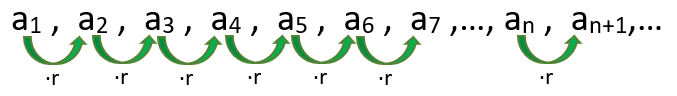
\includegraphics[width=0.75\textwidth]{successions.jpg}

    \vspace{4.5cm}
    \textbf{Professor:} Òscar Rodríguez \\
    \href{mailto:oscar.rodriguez@insjoseplladonosa.cat}{oscar.rodriguez@insjoseplladonosa.cat}
\end{titlepage}

\tableofcontents
\newpage

\hypersetup{pageanchor=true}
\pagenumbering{arabic}

% =========================================================
\section{Successions}

% ---------------------------------------------------------
\subsection{Concepte de successió}

\begin{concept}
\textbf{Definició de successió}\\
Una \textbf{successió} és una llista ordenada i infinita de nombres reals, on a cada nombre natural $n$ li correspon un nombre real $a_n$:
\[
a_1, a_2, a_3, a_4, \dots, a_n, \dots
\]
\begin{itemize}
    \item Cada $a_n$ s'anomena \textbf{terme} de la successió.
    \item El subíndex $n$ és la \textbf{posició} o índex del terme.
    \item El terme $a_n$ s'anomena \textbf{terme general} i permet calcular qualsevol terme de la successió.
\end{itemize}

\textbf{Tipus de successions:}
\begin{itemize}
    \item \textbf{Successió finita:} té un nombre limitat de termes, $a_1, a_2, \dots, a_k$.
    \item \textbf{Successió infinita:} té infinits termes, indicada per $\{a_n\}_{n \in \mathbb{N}}$.
\end{itemize}

Dues successions són iguals si tenen els mateixos termes en les mateixes posicions.
\end{concept}

\begin{exemple}
\textbf{Exemples de successions}
\begin{enumerate}[label=\alph*)]
    \item $2, 4, 6, 8, 10, \dots$ és la successió dels nombres parells. El terme general és $a_n = 2n$.
    \item $1, \dfrac{1}{2}, \dfrac{1}{3}, \dfrac{1}{4}, \dots$ té per terme general $a_n = \dfrac{1}{n}$.
    \item $1, 4, 9, 16, 25, \dots$ és la successió dels quadrats perfectes: $a_n = n^2$.
    \item $3, 3, 3, 3, \dots$ és una successió constant: $a_n = 3$.
\end{enumerate}
\end{exemple}

\begin{exercici}
\textbf{Exercici 1.1}\\
Escriu els cinc primers termes de cada successió donada pel seu terme general:
\begin{enumerate}[label=\alph*)]
    \item $a_n = 3n + 1$
    \item $a_n = n^2 - 1$
    \item $a_n = \dfrac{n+1}{n}$
    \item $a_n = (-1)^n \cdot n$
    \item $a_n = 2^n$
\end{enumerate}
\end{exercici}

% ---------------------------------------------------------
\subsection{Formes de definir una successió}

\begin{concept}
\textbf{Formes de definir una successió}\\
Hi ha dues maneres principals d'especificar una successió:

\textbf{1. Per la fórmula del terme general:}\\
Es dona una expressió $a_n = f(n)$ que permet calcular directament qualsevol terme a partir de la seva posició.
\[
a_n = f(n)
\]
Exemple: $a_n = 2n + 3 \implies a_5 = 2 \cdot 5 + 3 = 13$.

\textbf{2. Per recurrència:}\\
Es dona el primer terme (o els primers) i una fórmula que permet obtenir cada terme a partir dels anteriors.
\[
a_1 = \text{valor inicial}, \qquad a_{n+1} = f(a_n)
\]
Exemple: $a_1 = 1$, $a_{n+1} = a_n + 3$ \\
$\implies a_2 = 4, \ a_3 = 7, \ a_4 = 10, \dots$
\end{concept}

\begin{exemple}
\textbf{Successió definida per recurrència}
\[
a_1 = 2, \qquad a_{n+1} = 2 a_n + 1
\]
Calculem els primers termes:
\[
a_1 = 2, \quad a_2 = 2 \cdot 2 + 1 = 5, \quad a_3 = 2 \cdot 5 + 1 = 11, \quad a_4 = 2 \cdot 11 + 1 = 23, \dots
\]
\end{exemple}

\begin{exercici}
\textbf{Exercici 1.2}\\
Calcula els quatre primers termes de les successions definides per recurrència:
\begin{enumerate}[label=\alph*)]
    \item $a_1 = 3$, $a_{n+1} = a_n + 5$
    \item $a_1 = 1$, $a_{n+1} = 3 a_n$
    \item $a_1 = 1$, $a_2 = 1$, $a_{n+2} = a_{n+1} + a_n$ (successió de Fibonacci)
    \item $a_1 = 4$, $a_{n+1} = \dfrac{a_n}{2}$
\end{enumerate}
\end{exercici}

% ---------------------------------------------------------
\subsection{Successions monòtones i fitades}

\begin{concept}
\textbf{Monotonia}\\
Una successió $\{a_n\}$ és:
\begin{itemize}
    \item \textbf{Creixent} si $a_{n+1} > a_n$ per a tot $n$. Exemple: $1, 2, 3, 4, \dots$
    \item \textbf{Decreixent} si $a_{n+1} < a_n$ per a tot $n$. Exemple: $1, \tfrac{1}{2}, \tfrac{1}{3}, \dots$
    \item \textbf{Constant} si $a_{n+1} = a_n$ per a tot $n$. Exemple: $5, 5, 5, \dots$
\end{itemize}
Si és creixent o decreixent, diem que és \textbf{monòtona}.

\textbf{Fitació}\\
Una successió $\{a_n\}$ és:
\begin{itemize}
    \item \textbf{Fitada superiorment} si existeix un nombre $M$ tal que $a_n \le M$ per a tot $n$.
    \item \textbf{Fitada inferiorment} si existeix un nombre $m$ tal que $a_n \ge m$ per a tot $n$.
    \item \textbf{Fitada} si ho està superiorment i inferiorment alhora.
\end{itemize}
\end{concept}

\begin{exemple}
\textbf{Estudi de monotonia i fitació}
\begin{enumerate}[label=\alph*)]
    \item $a_n = n^2$: creixent, fitada inferiorment per $1$ (no superiorment).
    \item $a_n = \dfrac{1}{n}$: decreixent, fitada entre $0$ i $1$ ($0 < a_n \le 1$).
    \item $a_n = (-1)^n$: no és monòtona, però està fitada entre $-1$ i $1$.
    \item $a_n = 2n - 1$: creixent, fitada inferiorment per $1$ (no superiorment).
\end{enumerate}
\end{exemple}

\begin{exercici}
\textbf{Exercici 1.3}\\
Estudia la monotonia i la fitació de les següents successions:
\begin{enumerate}[label=\alph*)]
    \item $a_n = 3n - 2$
    \item $a_n = \dfrac{n+2}{n+1}$
    \item $a_n = -2n + 5$
    \item $a_n = (-1)^n \cdot \dfrac{1}{n}$
\end{enumerate}
\end{exercici}

% ---------------------------------------------------------
\subsection{Introducció al límit d'una successió}

\begin{concept}
\textbf{Idea intuïtiva de límit}\\
El \textbf{límit} d'una successió és el valor al qual s'aproximen els seus termes quan $n$ es fa molt gran. S'escriu:
\[
\lim_{n \to \infty} a_n = L
\]

\textbf{Tipus de successions segons el seu límit:}
\begin{itemize}
    \item \textbf{Convergent:} té un límit finit $L$. Exemple: $a_n = \dfrac{1}{n} \to 0$.
    \item \textbf{Divergent:} el límit és $+\infty$ o $-\infty$. Exemple: $a_n = n^2 \to +\infty$.
    \item \textbf{Oscil·lant o sense límit:} no tendeix a cap valor. Exemple: $a_n = (-1)^n$.
\end{itemize}

\textbf{Càlcul de límits senzills (regles intuïtives):}
\begin{itemize}
    \item Si $a_n$ és un polinomi de grau $k$, aleshores $\lim_{n\to\infty} a_n = \pm\infty$ segons el signe del coeficient principal.
    \item Si $a_n = \dfrac{P(n)}{Q(n)}$ amb polinomis, es compara el grau del numerador i del denominador:
    \begin{itemize}
        \item Grau numerador $<$ grau denominador $\Rightarrow$ límit $= 0$.
        \item Graus iguals $\Rightarrow$ límit $=$ quocient dels coeficients principals.
        \item Grau numerador $>$ grau denominador $\Rightarrow$ límit $=\pm\infty$.
    \end{itemize}
    \item Si $a_n = r^n$: si $|r| < 1$, $\lim_{n\to\infty} r^n = 0$; si $r > 1$, $= +\infty$.
\end{itemize}
\end{concept}

\begin{exemple}
\textbf{Càlcul de límits}
\begin{enumerate}[label=\alph*)]
    \item $\displaystyle\lim_{n\to\infty} \dfrac{1}{n} = 0$ (convergent).
    \item $\displaystyle\lim_{n\to\infty} \dfrac{3n+1}{2n-5} = \dfrac{3}{2}$ (convergent, graus iguals).
    \item $\displaystyle\lim_{n\to\infty} \dfrac{n^2+1}{n+3} = +\infty$ (divergent).
    \item $\displaystyle\lim_{n\to\infty} \left(\dfrac{1}{2}\right)^n = 0$ (convergent).
    \item $\displaystyle\lim_{n\to\infty} 2^n = +\infty$ (divergent).
\end{enumerate}
\end{exemple}

\begin{exercici}
\textbf{Exercici 1.4}\\
Calcula el límit de les següents successions i indica si són convergents o divergents:
\begin{enumerate}[label=\alph*)]
    \item $a_n = \dfrac{2n+3}{n+1}$
    \item $a_n = 5n^2 - 3n + 1$
    \item $a_n = \dfrac{3n^2 + 1}{n^2 + n}$
    \item $a_n = \left(\dfrac{3}{4}\right)^n$
    \item $a_n = \dfrac{(-1)^n}{n}$
\end{enumerate}
\end{exercici}

% ---------------------------------------------------------
% RESUM DEL BLOC 1
% ---------------------------------------------------------
\begin{resum}[title=Resum 1: Successions]
\textbf{Definicions bàsiques}
\[
a_1, a_2, a_3, \dots, a_n, \dots \quad \text{(terme general } a_n\text{)}
\]

\textbf{Formes de definir una successió}
\[
\text{Terme general: } a_n = f(n) \qquad \text{Recurrència: } a_{n+1} = f(a_n)
\]

\textbf{Monotonia i fitació}
\begin{itemize}
    \item Creixent: $a_{n+1} > a_n$ \quad Decreixent: $a_{n+1} < a_n$ \quad Constant: $a_{n+1} = a_n$
    \item Fitada: existeixen $m, M$ amb $m \le a_n \le M$ per a tot $n$.
\end{itemize}

\textbf{Límits (regles intuïtives)}
\[
\lim_{n\to\infty} \dfrac{1}{n} = 0, \qquad
\lim_{n\to\infty} \dfrac{an+b}{cn+d} = \dfrac{a}{c}, \qquad
\lim_{n\to\infty} r^n = \begin{cases} 0 & \text{si } |r|<1 \\ +\infty & \text{si } r>1 \end{cases}
\]
Convergent si el límit és finit; divergent si és $\pm\infty$; oscil·lant si no té límit.
\end{resum}

\newpage

% =========================================================
\section{Progressions Aritmètiques}

% ---------------------------------------------------------
\subsection{Definició i diferència}

\begin{concept}
\textbf{Definició de progressió aritmètica}\\
Una \textbf{progressió aritmètica} (PA) és una successió en què cada terme s'obté sumant al terme anterior una quantitat constant $d$, anomenada \textbf{diferència}.
\[
a_{n+1} = a_n + d \quad \text{per a tot } n
\]
La diferència es calcula com:
\[
d = a_{n+1} - a_n
\]

\textbf{Tipus segons la diferència:}
\begin{itemize}
    \item Si $d > 0$, la PA és \textbf{creixent}.
    \item Si $d < 0$, la PA és \textbf{decreixent}.
    \item Si $d = 0$, la PA és \textbf{constant}.
\end{itemize}
\end{concept}

\begin{figure}[H]
\centering
\begin{tikzpicture}[scale=1]
    \draw[->, thick] (-0.5,0) -- (10.5,0) node[right] {$\mathbb{R}$};
    \foreach \x/\lab in {0/{a_1}, 2/{a_2}, 4/{a_3}, 6/{a_4}, 8/{a_5}}
        \draw[thick] (\x,0.1) -- (\x,-0.1) node[below] {$\lab$};
    \foreach \x in {0,2,4,6}
        \draw[->, red, thick, dashed] (\x+0.15,0.3) to[bend left=20] (\x+1.85,0.3);
    \node[red, above] at (1,0.55) {$+d$};
    \node[red, above] at (3,0.55) {$+d$};
    \node[red, above] at (5,0.55) {$+d$};
    \node[red, above] at (7,0.55) {$+d$};
    \filldraw[blue] (0,0) circle (3pt);
    \filldraw[blue] (2,0) circle (3pt);
    \filldraw[blue] (4,0) circle (3pt);
    \filldraw[blue] (6,0) circle (3pt);
    \filldraw[blue] (8,0) circle (3pt);
\end{tikzpicture}
\caption{Una progressió aritmètica avança amb salts constants $d$.}
\end{figure}

\begin{exemple}
\textbf{Exemples de progressions aritmètiques}
\begin{enumerate}[label=\alph*)]
    \item $3, 7, 11, 15, 19, \dots$ és una PA amb $a_1 = 3$ i $d = 4$ (creixent).
    \item $20, 17, 14, 11, \dots$ és una PA amb $a_1 = 20$ i $d = -3$ (decreixent).
    \item $5, 5, 5, 5, \dots$ és una PA amb $d = 0$ (constant).
    \item $\dfrac{1}{2}, 1, \dfrac{3}{2}, 2, \dots$ és una PA amb $a_1 = \dfrac{1}{2}$ i $d = \dfrac{1}{2}$.
\end{enumerate}
\end{exemple}

\begin{exercici}
\textbf{Exercici 2.1}\\
Determina la diferència $d$ i digues si la progressió aritmètica és creixent o decreixent:
\begin{enumerate}[label=\alph*)]
    \item $2, 6, 10, 14, \dots$
    \item $100, 90, 80, 70, \dots$
    \item $\dfrac{1}{3}, \dfrac{2}{3}, 1, \dfrac{4}{3}, \dots$
    \item $-5, -8, -11, -14, \dots$
\end{enumerate}
\end{exercici}

% ---------------------------------------------------------
\subsection{Terme general}

\begin{concept}
\textbf{Terme general d'una PA}\\
El terme general d'una progressió aritmètica de primer terme $a_1$ i diferència $d$ és:
\[
\boxed{a_n = a_1 + (n-1) \, d}
\]

També es pot expressar en funció de qualsevol terme $a_k$:
\[
a_n = a_k + (n-k) \, d
\]

\textbf{Aïllaments útils:}
\[
d = \dfrac{a_n - a_1}{n-1}, \qquad n = \dfrac{a_n - a_1}{d} + 1
\]
\end{concept}

\begin{exemple}
\textbf{Càlcul de termes d'una PA}
\begin{enumerate}[label=\alph*)]
    \item A la PA $3, 7, 11, 15, \dots$, el terme general és $a_n = 3 + (n-1)\cdot 4 = 4n - 1$.
    \item El terme $a_{20}$ d'aquesta PA és $a_{20} = 4 \cdot 20 - 1 = 79$.
    \item Si $a_1 = 5$ i $a_{10} = 32$, la diferència és $d = \dfrac{32-5}{9} = 3$.
\end{enumerate}
\end{exemple}

\begin{exercici}
\textbf{Exercici 2.2}\\
Troba el terme general i el terme indicat:
\begin{enumerate}[label=\alph*)]
    \item $a_1 = 4$, $d = 3$. Calcula $a_{15}$.
    \item $a_1 = 10$, $d = -2$. Calcula $a_{12}$.
    \item $a_5 = 12$ i $a_{10} = 27$. Troba $a_1$ i $d$.
    \item La PA $7, 11, 15, \dots$. Quin és el terme $a_{25}$? És 103 un terme d'aquesta PA?
\end{enumerate}
\end{exercici}

% ---------------------------------------------------------
\subsection{Suma dels $n$ primers termes}

\begin{concept}
\textbf{Suma dels $n$ primers termes d'una PA}\\
La suma $S_n = a_1 + a_2 + \dots + a_n$ dels $n$ primers termes d'una PA es calcula amb una de les dues fórmules equivalents:
\[
\boxed{S_n = \dfrac{n(a_1 + a_n)}{2}}
\]
\[
\boxed{S_n = \dfrac{n \left[ 2a_1 + (n-1)d \right]}{2}}
\]

La primera fórmula s'usa quan es coneix l'últim terme; la segona quan només es coneix $a_1$ i $d$.
\end{concept}

\begin{exemple}
\textbf{Suma de termes d'una PA}
\begin{enumerate}[label=\alph*)]
    \item Suma dels 10 primers termes de la PA $3, 7, 11, \dots$:
    \[
    a_1 = 3, \quad d = 4 \implies a_{10} = 3 + 9 \cdot 4 = 39
    \]
    \[
    S_{10} = \dfrac{10(3+39)}{2} = \dfrac{10 \cdot 42}{2} = 210
    \]
    \item Suma dels 20 primers múltiples de 3: $a_1 = 3$, $d = 3$, $a_{20} = 60$.
    \[
    S_{20} = \dfrac{20(3+60)}{2} = 630
    \]
\end{enumerate}
\end{exemple}

\begin{exercici}
\textbf{Exercici 2.3}\\
Calcula les sumes següents:
\begin{enumerate}[label=\alph*)]
    \item Suma dels 15 primers termes de la PA $2, 5, 8, 11, \dots$
    \item Suma dels 20 primers termes de la PA $100, 95, 90, \dots$
    \item Suma dels primers 50 nombres naturals: $1 + 2 + 3 + \dots + 50$
    \item Suma de tots els múltiples de 7 menors que 100.
\end{enumerate}
\end{exercici}

% ---------------------------------------------------------
\subsection{Interpolació de termes aritmètics}

\begin{concept}
\textbf{Interpolació de termes aritmètics}\\
\textbf{Interpolar} $k$ termes aritmètics entre dos nombres $a$ i $b$ significa construir una PA de $k+2$ termes que comenci a $a$ i acabi a $b$:
\[
a, \ x_1, \ x_2, \ \dots, \ x_k, \ b
\]

La diferència s'obté dividint la distància total entre el nombre d'intervals:
\[
\boxed{d = \dfrac{b - a}{k + 1}}
\]

Els termes intermedis són:
\[
x_i = a + i \cdot d, \qquad i = 1, 2, \dots, k
\]
\end{concept}

\begin{exemple}
\textbf{Interpolació aritmètica}
Interpolar 3 termes aritmètics entre $2$ i $18$:
\[
d = \dfrac{18-2}{3+1} = \dfrac{16}{4} = 4
\]
Els termes són:
\[
2, \ 6, \ 10, \ 14, \ 18
\]
\end{exemple}

\begin{exercici}
\textbf{Exercici 2.4}\\
\begin{enumerate}[label=\alph*)]
    \item Interpola 4 termes aritmètics entre $5$ i $30$.
    \item Interpola 5 termes aritmètics entre $-8$ i $22$.
    \item Interpola 3 termes aritmètics entre $\dfrac{1}{2}$ i $\dfrac{9}{2}$.
\end{enumerate}
\end{exercici}

% ---------------------------------------------------------
% RESUM DEL BLOC 2
% ---------------------------------------------------------
\begin{resum}[title=Resum 2: Progressions Aritmètiques]
\textbf{Definició}
\[
a_{n+1} = a_n + d, \qquad d = a_{n+1} - a_n
\]

\textbf{Terme general}
\[
a_n = a_1 + (n-1)d
\]
\[
a_n = a_k + (n-k)d
\]

\textbf{Suma dels $n$ primers termes}
\[
S_n = \dfrac{n(a_1 + a_n)}{2} = \dfrac{n\left[2a_1 + (n-1)d\right]}{2}
\]

\textbf{Interpolació de $k$ termes entre $a$ i $b$}
\[
d = \dfrac{b-a}{k+1}
\]
\end{resum}

\newpage

% =========================================================
\section{Progressions Geomètriques}

% ---------------------------------------------------------
\subsection{Definició i raó}

\begin{concept}
\textbf{Definició de progressió geomètrica}\\
Una \textbf{progressió geomètrica} (PG) és una successió en què cada terme s'obté multiplicant el terme anterior per una quantitat constant $r$, anomenada \textbf{raó}.
\[
a_{n+1} = a_n \cdot r \quad \text{per a tot } n
\]
La raó es calcula com:
\[
r = \dfrac{a_{n+1}}{a_n} \quad (a_n \neq 0)
\]

\textbf{Tipus segons la raó:}
\begin{itemize}
    \item Si $r > 1$ i $a_1 > 0$, la PG és \textbf{creixent}.
    \item Si $0 < r < 1$ i $a_1 > 0$, la PG és \textbf{decreixent}.
    \item Si $r < 0$, la PG és \textbf{alternada} (canvia de signe).
    \item Si $r = 1$, la PG és \textbf{constant}.
\end{itemize}
\end{concept}

\begin{figure}[H]
\centering
\begin{tikzpicture}[scale=0.7]
    \draw[->, thick] (-0.5,0) -- (10.5,0) node[right] {$n$};
    \draw[->, thick] (0,-0.5) -- (0,9) node[above] {$a_n$};
    % Punts d'una PG amb a1=1, r=1.5: 1, 1.5, 2.25, 3.375, 5.06, 7.59
    \foreach \x/\y in {1/1, 2/1.5, 3/2.25, 4/3.375, 5/5.06, 6/7.59}
        \filldraw[blue] (\x,\y) circle (3pt);
    % Corba exponencial aproximada
    \draw[red, thick, smooth, domain=0.5:6.5, samples=50]
        plot (\x, {1.5^(\x-1)});
    \node[red, above] at (5.7,6.5) {$a_n = a_1 \cdot r^{n-1}$};
    \node[below] at (1,0) {\small $1$};
    \node[below] at (2,0) {\small $2$};
    \node[below] at (3,0) {\small $3$};
    \node[below] at (4,0) {\small $4$};
    \node[below] at (5,0) {\small $5$};
    \node[below] at (6,0) {\small $6$};
\end{tikzpicture}
\caption{Una progressió geomètrica creix exponencialment (cas $a_1 = 1$, $r = 1{,}5$).}
\end{figure}

\begin{exemple}
\textbf{Exemples de progressions geomètriques}
\begin{enumerate}[label=\alph*)]
    \item $2, 6, 18, 54, \dots$ és una PG amb $a_1 = 2$ i $r = 3$ (creixent).
    \item $80, 40, 20, 10, \dots$ és una PG amb $a_1 = 80$ i $r = \dfrac{1}{2}$ (decreixent).
    \item $3, -6, 12, -24, \dots$ és una PG amb $a_1 = 3$ i $r = -2$ (alternada).
    \item $5, 5, 5, 5, \dots$ és una PG amb $r = 1$ (constant).
\end{enumerate}
\end{exemple}

\begin{exercici}
\textbf{Exercici 3.1}\\
Determina la raó $r$ i digues si la progressió geomètrica és creixent, decreixent o alternada:
\begin{enumerate}[label=\alph*)]
    \item $1, 3, 9, 27, \dots$
    \item $64, 32, 16, 8, \dots$
    \item $5, -10, 20, -40, \dots$
    \item $\dfrac{1}{3}, \dfrac{1}{6}, \dfrac{1}{12}, \dots$
\end{enumerate}
\end{exercici}

% ---------------------------------------------------------
\subsection{Terme general}

\begin{concept}
\textbf{Terme general d'una PG}\\
El terme general d'una progressió geomètrica de primer terme $a_1$ i raó $r$ és:
\[
\boxed{a_n = a_1 \cdot r^{n-1}}
\]

També es pot expressar en funció de qualsevol terme $a_k$:
\[
a_n = a_k \cdot r^{n-k}
\]

\textbf{Aïllaments útils:}
\[
r = \sqrt[n-1]{\dfrac{a_n}{a_1}} \qquad (\text{si } a_1, a_n > 0)
\]
\end{concept}

\begin{exemple}
\textbf{Càlcul de termes d'una PG}
\begin{enumerate}[label=\alph*)]
    \item A la PG $2, 6, 18, 54, \dots$, el terme general és $a_n = 2 \cdot 3^{n-1}$.
    \item El terme $a_6$ és $a_6 = 2 \cdot 3^5 = 486$.
    \item Si $a_1 = 5$ i $a_4 = 40$, la raó és $r^3 = 8 \implies r = 2$.
\end{enumerate}
\end{exemple}

\begin{exercici}
\textbf{Exercici 3.2}\\
Troba el terme general i el terme indicat:
\begin{enumerate}[label=\alph*)]
    \item $a_1 = 3$, $r = 2$. Calcula $a_8$.
    \item $a_1 = 100$, $r = \dfrac{1}{2}$. Calcula $a_6$.
    \item $a_3 = 12$ i $a_6 = 96$. Troba $a_1$ i $r$.
    \item La PG $1, 4, 16, \dots$. És 1024 un terme d'aquesta PG? Quin lloc ocupa?
\end{enumerate}
\end{exercici}

% ---------------------------------------------------------
\subsection{Suma dels $n$ primers termes}

\begin{concept}
\textbf{Suma dels $n$ primers termes d'una PG}\\
La suma $S_n = a_1 + a_2 + \dots + a_n$ dels $n$ primers termes d'una PG amb $r \neq 1$ és:
\[
\boxed{S_n = \dfrac{a_n \cdot r - a_1}{r-1} = \dfrac{a_1 (r^n - 1)}{r-1}}
\]

Si $r = 1$, la PG és constant i $S_n = n \cdot a_1$.
\end{concept}

\begin{exemple}
\textbf{Suma de termes d'una PG}
\begin{enumerate}[label=\alph*)]
    \item Suma dels 5 primers termes de la PG $2, 6, 18, 54, 162$:
    \[
    S_5 = \dfrac{2(3^5 - 1)}{3-1} = \dfrac{2(243-1)}{2} = 242
    \]
    \item Suma dels 10 primers termes de la PG $1, \dfrac{1}{2}, \dfrac{1}{4}, \dots$:
    \[
    S_{10} = \dfrac{1\left[\left(\frac{1}{2}\right)^{10} - 1\right]}{\frac{1}{2}-1} = \dfrac{\frac{1}{1024}-1}{-\frac{1}{2}} = \dfrac{1023}{512}
    \]
\end{enumerate}
\end{exemple}

\begin{exercici}
\textbf{Exercici 3.3}\\
Calcula les sumes següents:
\begin{enumerate}[label=\alph*)]
    \item Suma dels 6 primers termes de la PG $3, 6, 12, 24, \dots$
    \item Suma dels 5 primers termes de la PG $1000, 100, 10, \dots$
    \item Suma dels 8 primers termes de la PG $1, -2, 4, -8, \dots$
    \item Una PG té $a_1 = 2$, $r = 3$. Calcula $S_{10}$.
\end{enumerate}
\end{exercici}

% ---------------------------------------------------------
\subsection{Suma dels infinits termes}

\begin{concept}
\textbf{Suma dels infinits termes}\\
Si $|r| < 1$, els termes d'una PG es fan cada vegada més petits (tendeixen a zero). En aquest cas, la suma de tots els infinits termes convergeix a un valor finit:
\[
\boxed{S_\infty = \dfrac{a_1}{1 - r} \quad \text{només si } |r| < 1}
\]

Si $|r| \ge 1$, la suma no convergeix (val $\pm\infty$ o no té límit).
\end{concept}

\begin{exemple}
\textbf{Suma infinita d'una PG}
\begin{enumerate}[label=\alph*)]
    \item $1 + \dfrac{1}{2} + \dfrac{1}{4} + \dfrac{1}{8} + \dots$ té $a_1 = 1$, $r = \dfrac{1}{2}$. Com $|r|<1$:
    \[
    S_\infty = \dfrac{1}{1 - \frac{1}{2}} = 2
    \]
    \item $3 + 1 + \dfrac{1}{3} + \dfrac{1}{9} + \dots$ té $a_1 = 3$, $r = \dfrac{1}{3}$:
    \[
    S_\infty = \dfrac{3}{1 - \frac{1}{3}} = \dfrac{3}{\frac{2}{3}} = \dfrac{9}{2} = 4{,}5
    \]
\end{enumerate}
\end{exemple}

\begin{exercici}
\textbf{Exercici 3.4}\\
Calcula la suma dels infinits termes, si és possible:
\begin{enumerate}[label=\alph*)]
    \item $2 + 1 + \dfrac{1}{2} + \dfrac{1}{4} + \dots$
    \item $8 + 4 + 2 + 1 + \dots$
    \item $1 - \dfrac{1}{3} + \dfrac{1}{9} - \dfrac{1}{27} + \dots$
    \item $5 + 10 + 20 + 40 + \dots$
\end{enumerate}
\end{exercici}

% ---------------------------------------------------------
\subsection{Producte dels $n$ primers termes}

\begin{concept}
\textbf{Producte dels $n$ primers termes d'una PG}\\
El producte $P_n = a_1 \cdot a_2 \cdot \dots \cdot a_n$ dels $n$ primers termes d'una PG es pot calcular com:
\[
\boxed{P_n = \sqrt{(a_1 \cdot a_n)^n}}
\]

\textbf{Idea intuïtiva:} Aquesta fórmula surt d'observar que els productes de parells de termes equidistants dels extrems són iguals: $a_1 \cdot a_n = a_2 \cdot a_{n-1} = \dots$
\end{concept}

\begin{exemple}
\textbf{Producte de termes d'una PG}
Producte dels 4 primers termes de la PG $2, 6, 18, 54$:
\[
P_4 = \sqrt{(2 \cdot 54)^4} = \sqrt{108^4} = 108^2 = 11664
\]
Comprovació directa: $2 \cdot 6 \cdot 18 \cdot 54 = 11664$. \checkmark
\end{exemple}

\begin{exercici}
\textbf{Exercici 3.5}\\
Calcula el producte dels primers termes indicats:
\begin{enumerate}[label=\alph*)]
    \item Producte dels 4 primers termes de la PG $1, 3, 9, 27$.
    \item Producte dels 5 primers termes de la PG $2, 4, 8, 16, 32$.
    \item Producte dels 3 primers termes de la PG $5, 10, 20$.
\end{enumerate}
\end{exercici}

% ---------------------------------------------------------
\subsection{Interpolació de termes geomètrics}

\begin{concept}
\textbf{Interpolació de termes geomètrics}\\
\textbf{Interpolar} $k$ termes geomètrics entre dos nombres $a$ i $b$ significa construir una PG de $k+2$ termes que comenci a $a$ i acabi a $b$:
\[
a, \ x_1, \ x_2, \ \dots, \ x_k, \ b
\]

La raó s'obté:
\[
\boxed{r = \sqrt[k+1]{\dfrac{b}{a}}}
\]

Els termes intermedis són:
\[
x_i = a \cdot r^i, \qquad i = 1, 2, \dots, k
\]
\end{concept}

\begin{exemple}
\textbf{Interpolació geomètrica}
Interpolar 3 termes geomètrics entre $2$ i $162$:
\[
r = \sqrt[4]{\dfrac{162}{2}} = \sqrt[4]{81} = 3
\]
Els termes són:
\[
2, \ 6, \ 18, \ 54, \ 162
\]
\end{exemple}

\begin{exercici}
\textbf{Exercici 3.6}\\
\begin{enumerate}[label=\alph*)]
    \item Interpola 3 termes geomètrics entre $1$ i $81$.
    \item Interpola 4 termes geomètrics entre $32$ i $1$.
    \item Interpola 2 termes geomètrics entre $5$ i $40$.
\end{enumerate}
\end{exercici}

% ---------------------------------------------------------
% RESUM DEL BLOC 3
% ---------------------------------------------------------
\begin{resum}[title=Resum 3: Progressions Geomètriques]
\textbf{Definició}
\[
a_{n+1} = a_n \cdot r, \qquad r = \dfrac{a_{n+1}}{a_n}
\]

\textbf{Terme general}
\[
a_n = a_1 \cdot r^{n-1} = a_k \cdot r^{n-k}
\]

\textbf{Suma dels $n$ primers termes} (per a $r \neq 1$)
\[
S_n = \dfrac{a_1(r^n-1)}{r-1} = \dfrac{a_n r - a_1}{r-1}
\]

\textbf{Suma dels infinits termes} (només si $|r|<1$)
\[
S_\infty = \dfrac{a_1}{1-r}
\]

\textbf{Producte dels $n$ primers termes}
\[
P_n = \sqrt{(a_1 \cdot a_n)^n}
\]

\textbf{Interpolació de $k$ termes entre $a$ i $b$}
\[
r = \sqrt[k+1]{\dfrac{b}{a}}
\]
\end{resum}

\newpage

% =========================================================
\section{Aplicacions i Problemes}

\begin{concept}
\textbf{Estratègia per resoldre problemes}\\
Davant d'un problema de successions o progressions, seguirem aquests passos:
\begin{enumerate}
    \item \textbf{Identificar el tipus}: és una PA o una PG?
    \begin{itemize}
        \item Si cada terme s'obté \emph{sumant} una quantitat fixa $\to$ PA.
        \item Si cada terme s'obté \emph{multiplicant} per una quantitat fixa $\to$ PG.
    \end{itemize}
    \item \textbf{Identificar les dades}: $a_1$, $d$ o $r$, $n$, $a_n$...
    \item \textbf{Aplicar la fórmula adequada}.
    \item \textbf{Comprovar} que la solució té sentit amb l'enunciat.
\end{enumerate}
\end{concept}

\begin{exemple}
\textbf{Problema resolt 1 (PA)}\\
Una empresa ven 500 unitats el primer mes i augmenta les vendes en 30 unitats cada mes. Quantes unitats vendrà el mes 12? Quantes n'haurà venut en total durant els 12 mesos?
\[
a_1 = 500, \quad d = 30 \implies a_{12} = 500 + 11 \cdot 30 = 830
\]
\[
S_{12} = \dfrac{12(500 + 830)}{2} = \dfrac{12 \cdot 1330}{2} = 7980
\]
L'empresa vendrà 830 unitats el mes 12 i 7980 unitats en total.
\end{exemple}

\begin{exemple}
\textbf{Problema resolt 2 (PG)}\\
Un estalviador diposita 200 € i cada any dobla el capital anterior. Quant tindrà al cap de 8 anys?
\[
a_1 = 200, \quad r = 2 \implies a_8 = 200 \cdot 2^7 = 200 \cdot 128 = 25600 \text{ €}
\]
Al cap de 8 anys tindrà 25\,600 €.
\end{exemple}

\begin{exemple}
\textbf{Problema resolt 3 (PG amb suma infinita)}\\
Una pilota cau des de 4 m d'alçada. A cada bot, rebota fins a $\dfrac{3}{4}$ de l'alçada anterior. Quina distància total haurà recorregut quan s'aturi?
\[
\text{Bot 1: } 4, \quad \text{Bot 2: } 4 \cdot \dfrac{3}{4}, \quad \text{Bot 3: } 4 \cdot \left(\dfrac{3}{4}\right)^2, \dots
\]
La distància total (pujada i baixada) és:
\[
d = 4 + 2 \cdot \left[ 4 \cdot \dfrac{3}{4} + 4 \cdot \left(\dfrac{3}{4}\right)^2 + \dots \right] = 4 + 2 \cdot \dfrac{3}{1 - \frac{3}{4}} = 4 + 2 \cdot 12 = 28 \text{ m}
\]
\end{exemple}

\begin{exercici}
\textbf{Exercici 4.1}\\
Un teatre té 20 files de seients. La primera fila té 15 seients, la segona 17, la tercera 19, i així successivament. Quants seients té l'última fila? Quants seients té el teatre en total?
\end{exercici}

\begin{exercici}
\textbf{Exercici 4.2}\\
El sou inicial d'un treballador és de 18\,000 € anuals i s'incrementa 500 € cada any. Quant cobrarà el 10è any? Quants diners haurà cobrat en total durant els 10 anys?
\end{exercici}

\begin{exercici}
\textbf{Exercici 4.3}\\
Una població de bacteris es triplica cada hora. Si inicialment hi ha 100 bacteris, quants n'hi haurà al cap de 6 hores?
\end{exercici}

\begin{exercici}
\textbf{Exercici 4.4}\\
Un cotxe es deprecia un 15\% anual. Si el seu valor inicial és de 20\,000 €, quin serà el seu valor al cap de 5 anys?
\emph{(Indicació: cada any el valor es multiplica per $0{,}85$.)}
\end{exercici}

\begin{exercici}
\textbf{Exercici 4.5}\\
En un quadrat de costat 1, s'inscriu un altre quadrat unint els punts mitjans dels costats, i així successivament. Quina és la suma de les àrees de tots els quadrats infinits?
\emph{(Indicació: cada quadrat té àrea meitat de l'anterior.)}
\end{exercici}

% ---------------------------------------------------------
% RESUM DEL BLOC 4
% ---------------------------------------------------------
\begin{resum}[title=Resum 4: Aplicacions]
\textbf{Passos per resoldre problemes}
\begin{enumerate}
    \item Identificar si és una PA (suma constant) o una PG (producte constant).
    \item Extreure les dades: $a_1$, $d$ o $r$, $n$.
    \item Aplicar la fórmula del terme general o de la suma.
    \item Comprovar que la solució té sentit.
\end{enumerate}

\textbf{Pistes útils}
\begin{itemize}
    \item Paraules com «augmenta en», «cada any +», «diferència» $\to$ PA.
    \item Paraules com «es multiplica per», «es dobla», «percentatge acumulat» $\to$ PG.
    \item Si el problema parla de sumar infinits termes decreixents, sovint cal usar $S_\infty = \dfrac{a_1}{1-r}$.
\end{itemize}
\end{resum}

\newpage

% =========================================================
% SOLUCIONS
% =========================================================
\appendix
\section{Solucions dels Exercicis Proposats}

\begin{solucio}
\textbf{Solucions de l'Apartat 1: Successions}
\begin{itemize}
    \item \textbf{Exercici 1.1:}
    \begin{enumerate}[label=\alph*)]
        \item $4, 7, 10, 13, 16$
        \item $0, 3, 8, 15, 24$
        \item $\dfrac{2}{1}, \dfrac{3}{2}, \dfrac{4}{3}, \dfrac{5}{4}, \dfrac{6}{5}$
        \item $-1, 2, -3, 4, -5$
        \item $2, 4, 8, 16, 32$
    \end{enumerate}
    \item \textbf{Exercici 1.2:}
    \begin{enumerate}[label=\alph*)]
        \item $3, 8, 13, 18$
        \item $1, 3, 9, 27$
        \item $1, 1, 2, 3$ (Fibonacci)
        \item $4, 2, 1, \dfrac{1}{2}$
    \end{enumerate}
    \item \textbf{Exercici 1.3:}
    \begin{enumerate}[label=\alph*)]
        \item Creixent, fitada inferiorment per $1$.
        \item Decreixent, fitada entre $1$ i $\dfrac{3}{2}$ (aproximadament). En general, $1 < a_n \le \dfrac{3}{2}$.
        \item Decreixent, fitada superiorment per $3$.
        \item No monòtona (oscil·lant), fitada entre $-\dfrac{1}{2}$ i $\dfrac{1}{2}$.
    \end{enumerate}
    \item \textbf{Exercici 1.4:}
    \begin{enumerate}[label=\alph*)]
        \item $\lim = 2$, convergent.
        \item $\lim = +\infty$, divergent.
        \item $\lim = 3$, convergent.
        \item $\lim = 0$, convergent.
        \item $\lim = 0$, convergent.
    \end{enumerate}
\end{itemize}
\end{solucio}

\begin{solucio}
\textbf{Solucions de l'Apartat 2: Progressions Aritmètiques}
\begin{itemize}
    \item \textbf{Exercici 2.1:}
    \begin{enumerate}[label=\alph*)]
        \item $d = 4$, creixent.
        \item $d = -10$, decreixent.
        \item $d = \dfrac{1}{3}$, creixent.
        \item $d = -3$, decreixent.
    \end{enumerate}
    \item \textbf{Exercici 2.2:}
    \begin{enumerate}[label=\alph*)]
        \item $a_n = 4 + 3(n-1) = 3n + 1$. $a_{15} = 46$.
        \item $a_n = 10 - 2(n-1) = 12 - 2n$. $a_{12} = -12$.
        \item $d = \dfrac{27-12}{5} = 3$; $a_1 = 12 - 4 \cdot 3 = 0$.
        \item $a_n = 7 + 4(n-1) = 4n + 3$. $a_{25} = 103$. Sí, el 103 és el terme $a_{25}$.
    \end{enumerate}
    \item \textbf{Exercici 2.3:}
    \begin{enumerate}[label=\alph*)]
        \item $a_{15} = 2 + 14 \cdot 3 = 44$; $S_{15} = \dfrac{15(2+44)}{2} = 345$.
        \item $a_{20} = 100 - 19 \cdot 5 = 5$; $S_{20} = \dfrac{20(100+5)}{2} = 1050$.
        \item $S_{50} = \dfrac{50 \cdot 51}{2} = 1275$.
        \item Múltiples de 7 menors que 100: $7, 14, \dots, 98$. $n = 14$, $S = \dfrac{14(7+98)}{2} = 735$.
    \end{enumerate}
    \item \textbf{Exercici 2.4:}
    \begin{enumerate}[label=\alph*)]
        \item $d = \dfrac{30-5}{5} = 5 \implies 5, 10, 15, 20, 25, 30$.
        \item $d = \dfrac{22-(-8)}{6} = 5 \implies -8, -3, 2, 7, 12, 17, 22$.
        \item $d = \dfrac{\frac{9}{2} - \frac{1}{2}}{4} = 1 \implies \dfrac{1}{2}, \dfrac{3}{2}, \dfrac{5}{2}, \dfrac{7}{2}, \dfrac{9}{2}$.
    \end{enumerate}
\end{itemize}
\end{solucio}

\begin{solucio}
\textbf{Solucions de l'Apartat 3: Progressions Geomètriques}
\begin{itemize}
    \item \textbf{Exercici 3.1:}
    \begin{enumerate}[label=\alph*)]
        \item $r = 3$, creixent.
        \item $r = \dfrac{1}{2}$, decreixent.
        \item $r = -2$, alternada.
        \item $r = \dfrac{1}{2}$, decreixent.
    \end{enumerate}
    \item \textbf{Exercici 3.2:}
    \begin{enumerate}[label=\alph*)]
        \item $a_n = 3 \cdot 2^{n-1}$; $a_8 = 3 \cdot 128 = 384$.
        \item $a_n = 100 \cdot \left(\dfrac{1}{2}\right)^{n-1}$; $a_6 = \dfrac{100}{32} = \dfrac{25}{8} = 3{,}125$.
        \item $r^3 = \dfrac{96}{12} = 8 \implies r = 2$; $a_1 = \dfrac{12}{4} = 3$.
        \item $a_n = 4^{n-1}$. $1024 = 4^5 \implies n-1 = 5 \implies n = 6$. Sí, és el terme $a_6$.
    \end{enumerate}
    \item \textbf{Exercici 3.3:}
    \begin{enumerate}[label=\alph*)]
        \item $S_6 = \dfrac{3(2^6-1)}{2-1} = 3 \cdot 63 = 189$.
        \item $S_5 = \dfrac{1000\left[\left(\frac{1}{10}\right)^5 - 1\right]}{\frac{1}{10}-1} = \dfrac{1000 \cdot \left(\frac{1}{100000} - 1\right)}{-\frac{9}{10}} = \dfrac{1000 \cdot \frac{-99999}{100000}}{-\frac{9}{10}} = 1111$.
        \item $S_8 = \dfrac{1 \cdot [(-2)^8 - 1]}{-2-1} = \dfrac{255}{-3} = -85$.
        \item $S_{10} = \dfrac{2(3^{10}-1)}{3-1} = 3^{10} - 1 = 59048$.
    \end{enumerate}
    \item \textbf{Exercici 3.4:}
    \begin{enumerate}[label=\alph*)]
        \item $a_1 = 2$, $r = \dfrac{1}{2}$. $S_\infty = \dfrac{2}{1 - \frac{1}{2}} = 4$.
        \item $a_1 = 8$, $r = \dfrac{1}{2}$. $S_\infty = \dfrac{8}{1 - \frac{1}{2}} = 16$.
        \item $a_1 = 1$, $r = -\dfrac{1}{3}$. $S_\infty = \dfrac{1}{1 + \frac{1}{3}} = \dfrac{3}{4}$.
        \item $r = 2 > 1$. La suma no convergeix.
    \end{enumerate}
    \item \textbf{Exercici 3.5:}
    \begin{enumerate}[label=\alph*)]
        \item $P_4 = \sqrt{(1 \cdot 27)^4} = 27^2 = 729$.
        \item $P_5 = \sqrt{(2 \cdot 32)^5} = \sqrt{64^5} = 64^{2{,}5} = 32768$.
        \item $P_3 = \sqrt{(5 \cdot 20)^3} = \sqrt{100^3} = 1000$.
    \end{enumerate}
    \item \textbf{Exercici 3.6:}
    \begin{enumerate}[label=\alph*)]
        \item $r = \sqrt[4]{81} = 3 \implies 1, 3, 9, 27, 81$.
        \item $r = \sqrt[5]{\dfrac{1}{32}} = \dfrac{1}{2} \implies 32, 16, 8, 4, 2, 1$.
        \item $r = \sqrt[3]{\dfrac{40}{5}} = 2 \implies 5, 10, 20, 40$.
    \end{enumerate}
\end{itemize}
\end{solucio}

\begin{solucio}
\textbf{Solucions de l'Apartat 4: Aplicacions}
\begin{itemize}
    \item \textbf{Exercici 4.1:} PA amb $a_1 = 15$, $d = 2$, $n = 20$. \\
    $a_{20} = 15 + 19 \cdot 2 = 53$ seients a l'última fila. \\
    $S_{20} = \dfrac{20(15+53)}{2} = 680$ seients en total.
    
    \item \textbf{Exercici 4.2:} PA amb $a_1 = 18000$, $d = 500$. \\
    $a_{10} = 18000 + 9 \cdot 500 = 22500$ € el 10è any. \\
    $S_{10} = \dfrac{10(18000+22500)}{2} = 202500$ € en total.
    
    \item \textbf{Exercici 4.3:} PG amb $a_1 = 100$, $r = 3$. \\
    $a_7 = 100 \cdot 3^6 = 72900$ bacteris (després de 6 hores, és el terme $a_7$). \\
    \emph{Nota: si comencem a comptar com a hora 0, al cap de 6 hores és $a_7$; si considerem $a_1$ com l'hora 1, aleshores és $a_7$ igualment. Revisar conveni.}
    
    \item \textbf{Exercici 4.4:} PG amb $a_1 = 20000$, $r = 0{,}85$. \\
    $a_6 = 20000 \cdot 0{,}85^5 = 20000 \cdot 0{,}4437 \approx 8874 \text{ €}$. \\
    \emph{(A l'any 5, terme $a_6$.)}
    
    \item \textbf{Exercici 4.5:} PG amb $a_1 = 1$, $r = \dfrac{1}{2}$. \\
    $S_\infty = \dfrac{1}{1 - \frac{1}{2}} = 2$ unitats quadrades.
\end{itemize}
\end{solucio}

\end{document}